\begin{figure}[H]
    \centering
    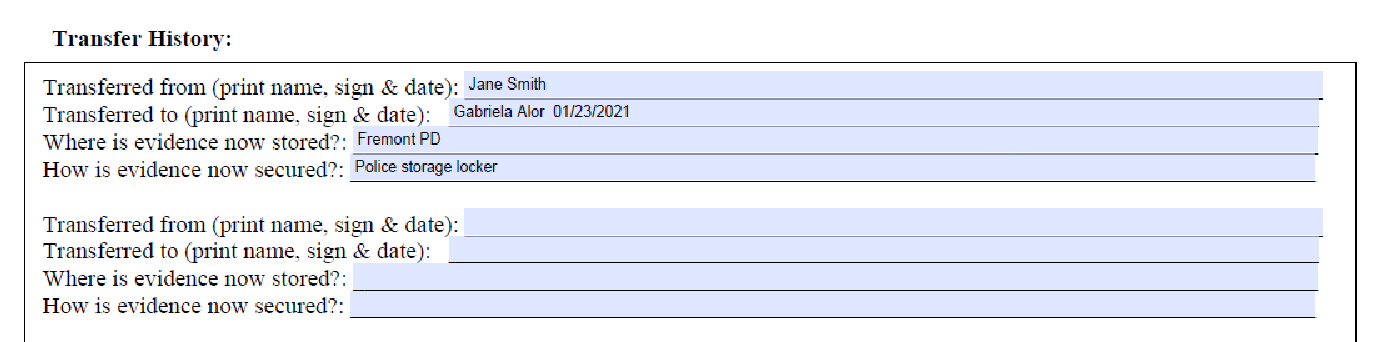
\includegraphics[width=\linewidth]{figures/Chain of Custody.png}
    \caption{Chain of Custody PDF.}
    \label{fig:coc}
\end{figure}
The chain of Custody file shows that we received evidence from Jane Smith on 1/23/2021 at the Fremont PD stored in a locker.

\begin{figure}[H]
    \centering
    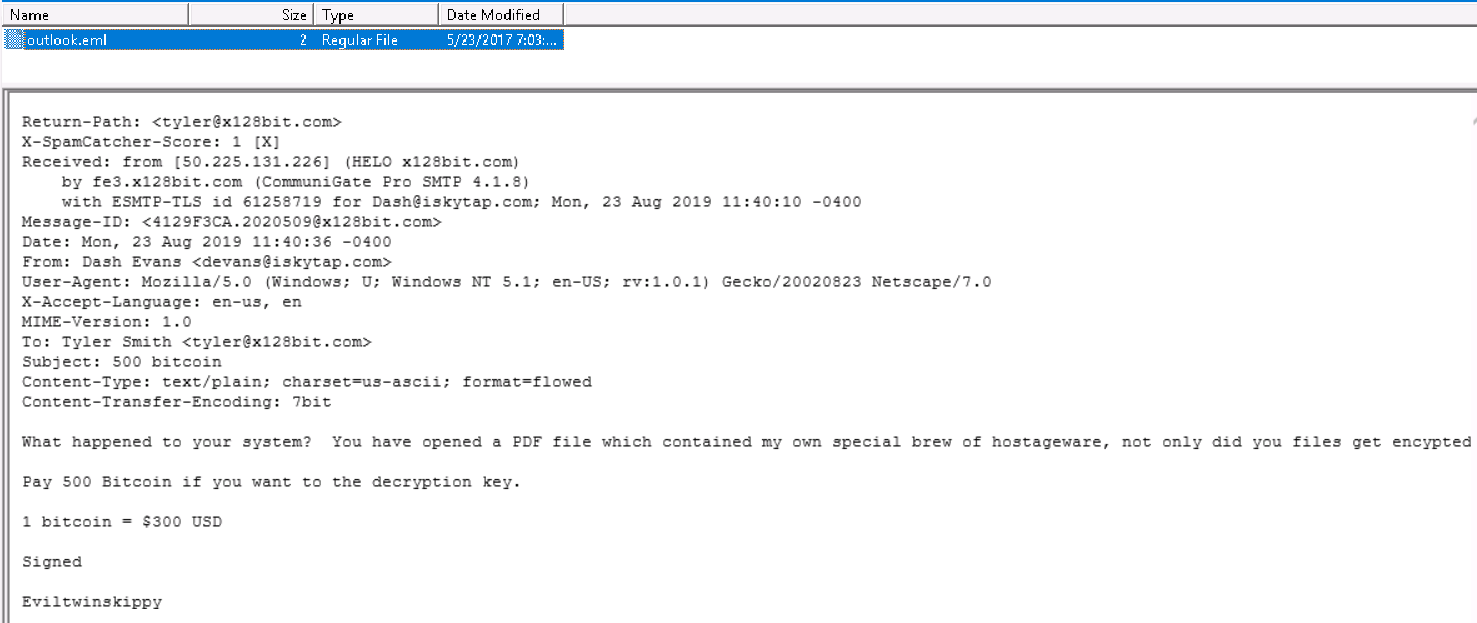
\includegraphics[width=\linewidth]{figures/outlook.eml.png}
    \caption{Contents of incriminating email.}
    \label{fig:email}
\end{figure}
The email shows extortion using ransomware to encrypt files, with the exchange of bitcoins for the decryption key.

\begin{figure}[H]
    \centering
    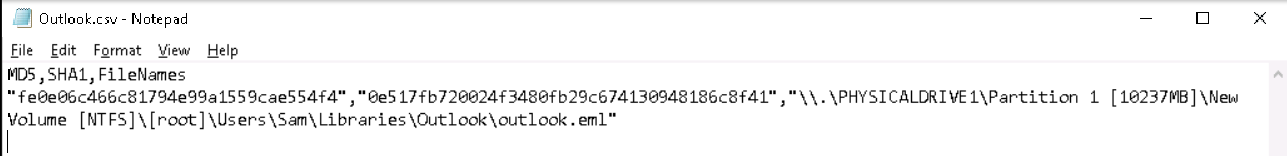
\includegraphics[width=\linewidth]{figures/outlook.csv.png}
    \caption{Hash value of the original Outlook file.}
    \label{fig:oHash}
\end{figure}

\begin{figure}[H]
    \centering
    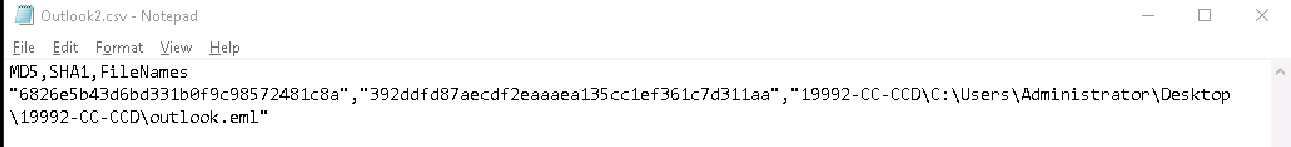
\includegraphics[width=\linewidth]{figures/outlook2.csv.png}
    \caption{Hash value of the altered Outlook file.}
    \label{fig:aHash}
\end{figure}

The hash values of these two files are different.
This indicates that the contents of these files are not the same.

\begin{figure}[H]
    \centering
    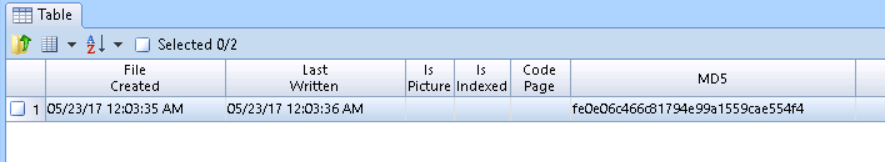
\includegraphics[width=\linewidth]{figures/md5.png}
    \caption{EnCase MD5 hash value for the Outlook file.}
    \label{fig:encase}
\end{figure}

\textbf{14.\ Question:} Describe how the hash value produced by EnCase Imager compares to the values produced by FTK Imager for the two Outlook files.\\
The EnCase MD5 hash value is the same as the MD5 produced by  FTK Imager for the original Outlook file.

\begin{figure}[H]
    \centering
    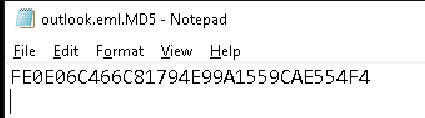
\includegraphics[width=\linewidth]{figures/outlook.eml.md5.png}
    \caption{E3 MD5 hash value for the Outlook file.}
    \label{fig:e3}
\end{figure}

\textbf{8.\ Question:} Describe how the hash value produced by E3 compares to the values produced by FTK Imager for the two Outlook files and the value produced by EnCase.\\
The hash produced by E3 is the same as the hash produced by FTK Imager for the first Outlook file and the MD5 generated by EnCase.
\newpage
In this lab we learned about how warrants are issued and the documentation of chain of custody to track who handles evidence.
We used three different evidence viewing programs, FTK Imager, Encase Imager and E3 to view evidence data and generate hash values.
Data can be pulled from many sources, including unallocated space on physical drives.
Because this unallocated space is used to store deleted files, this is typically a good place to check for evidence.
Hash values are used to validate that the evidence was not altered during the extraction process.
The Daubert standard states that the evidence files gathered were not altered by the forensic process.
In this case the hash of the original email matches the final hash generated, whereas the hash of the altered email is different.